\documentclass[a4paper, 12pt]{article}
% math symbols
\usepackage{amssymb}
\usepackage{amsmath}
\usepackage{mathrsfs}
\usepackage{physsummer}


\usepackage{enumitem}
\usepackage[margin = 2cm]{geometry}

\tolerance = 1000
\emergencystretch = 0.74cm



\pagestyle{empty}
\parindent = 0mm

\begin{document}

\begin{center}
  \Large{\textbf{Городской центр физического образования, 10 класс.}\\
  \textit{Серия 17, 12 февраля 2015.}}
\end{center}

\begin{center}
  \large\textbf{ Быстрая подготовка к городскому туру. }
\end{center}

\task{ Симметричная шляпа состоит из полусферы и полей постоянной
  ширины (см рис. слева). Её надевают на вешалку --- вертикальную
  палку с закругленным концом (см рис. справа, вид сбоку). Шляпу
  повесили таким образом, что угол $\alpha$, который её поля образуют
  с горизонталью, максимально возможный. Определите по рисунку
  коэффициент трения шляпы о вешалку. Считайте, что шляпа не
  деформируется. }
\begin{center}
  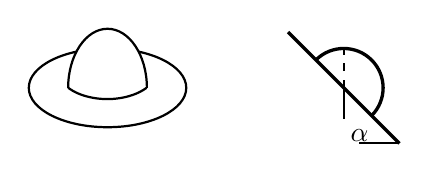
\begin{tikzpicture}
    \draw[thick] (0,0) ellipse (1cm and 0.5cm);
    \draw[thick,fill=white] (0.5,0) arc (0:180:0.5cm and 0.75cm);
    \draw[thick] (-0.5,0) arc (220:320:0.65cm and 0.4cm);
    \begin{scope}[xshift=2cm]
      \begin{scope}[rotate around={-45:(1,0)}]
        \draw[very thick] (0,0) -- (2,0);
        \draw[very thick] (0.5,0) arc (180:0:0.5cm);
      \end{scope}
      \draw[thick] (1,0) -- ++(0,-0.4);
      \draw[thick,dashed] (1,0) -- ++(0,0.5);
      \draw (1.7,-0.7) -- ++(-0.5,0) node[above=-0.1cm] {$\alpha$}; 
    \end{scope}
  \end{tikzpicture}
\end{center}

\task{ Бесконечная электрическая цепочка, изображенная на рисунке
  внизу, состоит из одинаковых идеальных сопротивлений $R$ и элементов
  \textbf{D} (идеальных диодов). Идеальный диод пропускает ток без
  сопротивления, если ток течет по <<стрелке>>, и не пропускает ток в
  обратном направлении. Экспериментатор стал исследовать зависимость
  напряжения между точками \textbf{A} и \textbf{B} от протекающего
  через схему полного тока, полученная им вольт-амперная
  характеристика приведена на графике справа (за положительное
  направление тока выбрано направление от точки \textbf{B} к точке
  \textbf{A}). Определите величину сопротивления $R$. }
\begin{center}
  \includegraphics[width=14cm]{1202151}
\end{center}

\taskpic{ В системе, изображенной на рисунке, $\nu$ молей идеального газа
  находятся в трубе сложной формы между тремя поршнями, каждый из
  которых может двигаться горизонтально по трубе без трения. Левый
  поршень имеет площадь $3S$, поршни справа имеют площади $S$ и $2S$,
  массы всех поршней одинаковы. Снаружи системы находится воздух при
  атмосферном давлении $p_0$ и температуре $T_0$. Поршни $3S$ и $S$
  скреплены пружиной жесткости $k$. Поршни $3S$ и $2S$ связаны
  нерастяжимой нитью, перекинутой через систему блоков, первоначально
  нить натянута до натяжения $F$. Нить перерезают. На сколько
  сдвинется каждый поршень, когда газ в сосуде придет в равновесие?
  Газ в трубе поддерживается при постоянной температуре
  $T_{0}$. Массами газа, пружины и нити пренебречь.  }
{
  \includegraphics[width=4cm]{1202152}
}

\end{document}


%%% Local Variables: 
%%% mode: latex
%%% TeX-engine:xetex
%%% TeX-PDF-mode: t
%%% End:
